\chapter{Printer Labels}
\label{chap:printer_labels}

The BioBank Java client can be used to print labels to any type of printer. At
the moment only \emph{CBSR Patient Labels} are supported.

\section{Patient Labels}
\label{sec:printer_labels}

\begin{wrapfigure}{r}{0.5\textwidth}
  \vspace{-20pt}
  \begin{center}
    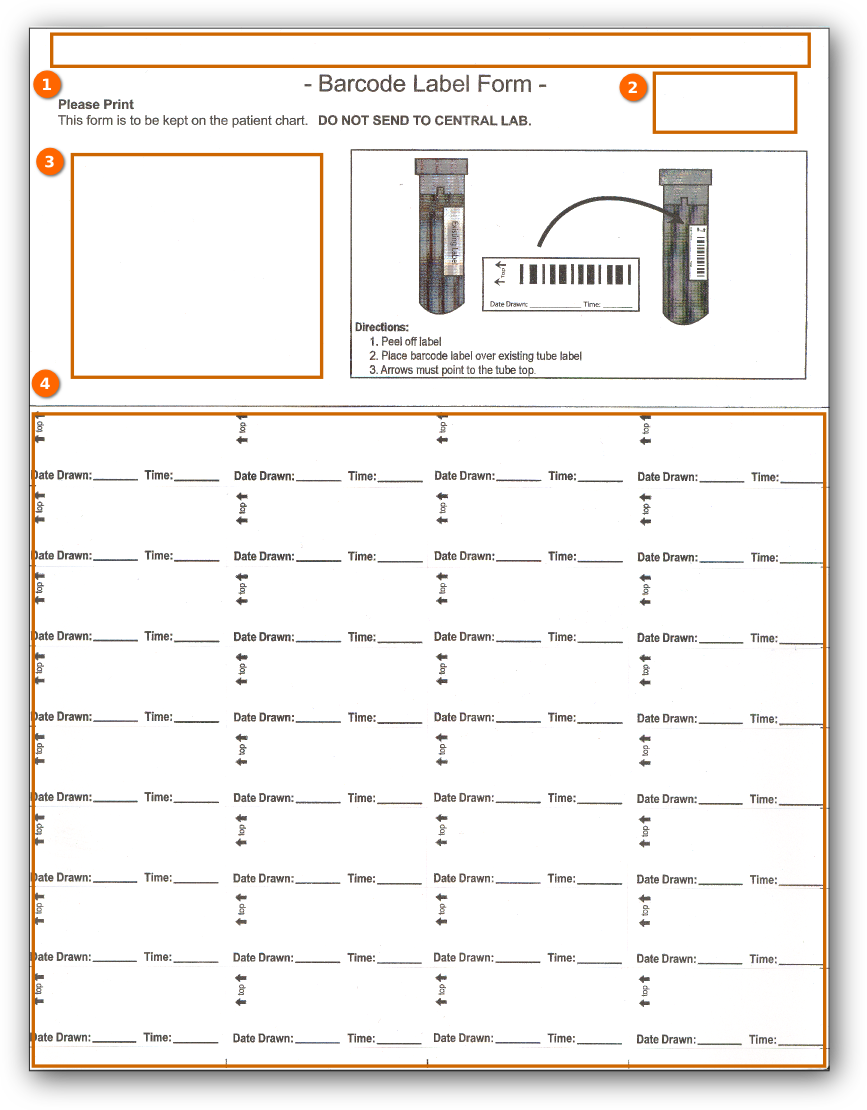
\includegraphics[width=0.5\textwidth]{screenshots/printer_labels/01_cbsr_patient_label_sheet}
  \end{center}
  \caption{CBSR Patient Label sheet.}
  \label{fig:cbsr_patient_label_sheet}
  \vspace{-15pt}
\end{wrapfigure}

Each patient label contains a 1D barcode for the patient number and a unique 2D
Data Matrix barcode for the specimen ID. Each specimen ID is unique amongst any
patient labels printed in the past and in the future. Also, the specimen ID is
unique across patients such that two patients will never have the same specimen
ID.

Figure \ref{fig:cbsr_patient_label_sheet} shows a blank CBSR Patient Label
sheet. It is a letter sized, 8$\frac{1}{2}$'' x 11'', sheet that
feeds into any printer.

The regions highlighted in orange are:
\begin{enumerate}
  \item The title area. Clinics and sites can customize their labels by
    printing their own title text.
  \item The logo region. A custom logo or graphic can be printed on the label.
  \item Patient information section. Up to 3 custom fields can be printed in
    this region.
  \item The individual patient labels that contain a 1D barcode for the patient
    number and a 2D barcode for the specimen ID. There are 32 labels in total.
\end{enumerate}

\subsection{Patient Label Information}

To print one of these sheets, some information must first be entered. Select
\texttt{Printer Labels} $\to$ \texttt{Patient Labels} from the main menu.

\begin{figure}[H]
  \centering
  \scalebox{0.35}
	   { \includegraphics*{screenshots/printer_labels/02_patient_labels_menu_item} }
	   \caption{Patient Labels menu item.}
	   \label{fig:patient_labels_menu_item}
\end{figure}

Figure \ref{fig:patient_label_form} shows the form that is displayed.

\begin{figure}[H]
  \centering
  \scalebox{0.45}
	   { \includegraphics*{screenshots/printer_labels/03_patient_label_form} }
	   \caption{Patient Label entry form.}
	   \label{fig:patient_label_form}
\end{figure}

In the \textbf{branding section}, the following information should be entered.

\begin{description}
\item[Title] This is the string that will be printed in the label sheet's title
  area. See area \textbf{1} in figure \ref{fig:cbsr_patient_label_sheet}. This field
  is optional.
\item[Logo] This allows you to select a graphic logo to be printed on the
  sheet. Press the \fbox{Browse} button to select the graphic file from your
  computer. This field is optional.
\item[Template] This is the template that specifies the position and dimension
  information for where to print information on the sheet. See section
  \ref{sec:label_templates} for more information on templates. The template
  name is a \textbf{required} field.
\item[Intended Printer] this is the printer the template was created for. You
  may have more than one template to select from. Each template is meant for a
  specific printer. This is displayed for informational purposes only.
\item[Printer] This pull down menu allows you to select the printer to use when
  printing the sheets. This menu displays the printers that have been
  configured on your computer. The printer is a \textbf{required} field.
\end{description}

In the \textbf{Patient Information} section the following information should be
entered.

\begin{description}
\item[Patient Number] Type the patient's number into this box. Any characters
  can be used up to a maximum of 14. This field cannot be left empty.
\item[Custom Fields] Three custom fields can be enabled to print on the
  label sheet. The text box on the left is the field name and the text box on
  the right is its corresponding value. In this example, the following are used
  for custom fields:

  \begin{center}
    \begin{tabular}{ | l | l | l | p{5cm} |}
      \hline
      Custom Field & Name & Value \\ \hline
      1 & Patient Name & Jonh Doe \\ \hline
      2 & PHN & 5555-5555-5555 \\ \hline
      3 & Patient Type & Control Patient \\
      \hline
    \end{tabular}
  \end{center}

  The checkboxes to the left of the field name can be used to enable / disable
  the printing of the field. The checkboxes in the middle are used to enable /
  disable printing of the value. The checkboxes on the right are used to enable
  / disable printing a 1D barcode for the corresponding field value. For
  example a 1D barcode will be printed with the text \emph{John Doe} encoded on
  it.
\end{description}

The above two sections are printed on the top portion of the label
sheet. Figure \ref{fig:printed_sheet_top} show what is printed for the values
entered into the form in figure \ref{fig:patient_label_form}.

\begin{figure}[H]
  \centering
  \scalebox{0.6}
	   { \includegraphics*{screenshots/printer_labels/04_printed_patient_labels_top} }
	   \caption{Top portion of printed patient label sheet.}
	   \label{fig:printed_sheet_top}
\end{figure}

The \textbf{Additional Configuration} section is for text to print under the
barcodes on each patient label. In the example shown in figure
\ref{fig:patient_label_form} the text \emph{Sp. Type} with underscore
characters will be printed as shown in \ref{fig:sp_type_single_label}.

\begin{figure}[H]
  \centering
  \scalebox{1.0}
	   { \includegraphics*{screenshots/printer_labels/05_single_label} }
	   \caption{Text printed on each label.}
	   \label{fig:sp_type_single_label}
\end{figure}

To print a sheet of labels you can press the \textbf{Print} button at the top
left of the form. Alternatively, instead of printing a sheet you can export the
sheet to a PDF file by pressing the \fbox{Export to PDF} button.

\subsection{Label Templates}
\label{sec:label_templates}

Select \texttt{Printer Labels} $\to$ \texttt{Label Templates} from the main
menu to see the form shown in figure \ref{fig:label_templates_form}.

\begin{figure}[H]
  \centering
  \scalebox{0.45}
	   { \includegraphics*{screenshots/printer_labels/06_label_templates_form} }
	   \caption{Label templates form.}
	   \label{fig:label_templates_form}
\end{figure}

The label template \emph{Patient with Source Specimen Label Template} is
already configured on the server for all users. This default template
tells the software where to print the information on the label sheet.  For your
printer, it is possible that the default template does not print the information
at the correct positions. You can create a new template by copying the default
template and adjusting the settings for your printer.

You may need to define templates for each printer that your computer can
access. To copy a template select the template you want to copy and press the
\fbox{Copy} button. You can also create a fresh template by pressing the
\fbox{New} button. In the future, you may want to delete an old template that
is no longer in use. This can be done by selecting the template to be deleted
and pressing the \fbox{Delete} button. To save your settings to the template
you can press the \textbf{Confirm} button at the top left of the form.

The settings for a template are:
\begin{description}
\item[Template Name] A descriptive name for the template. It is a good idea to
  include the name of the printer the template is intended for.
\item[Jasper Configuration] For patient labels you should always select the
\emph{Patient with Source Specimens Jasper Template}. This template is defined
by default on the server. For more information see section \ref{sec:jasper_templates}.
\item[Intended Printer] the name of the printer the template is intended for.
\item[Configuration] Allows for adjustments to the positions for the items to be printed.
\end{description}

Each 1D and 2D barcode item on the sheet has a \textbf{horizontal offset},
\textbf{vertical offset}, \textbf{width} and \textbf{height}. All measurements
are in millimetres. The \textbf{Patient Info} group corresponds to section
\textbf{3} in figure \ref{fig:cbsr_patient_label_sheet}. The \textbf{Barcodes}
group corresponds to the 32 patient labels. The labels are numbered starting at
the top left and ending at the bottom right. Under this group there is a
\textbf{General} node that controls the position of the patient 1D barcode, the
specimen ID 2D barcode, and the custom text position for all 32 labels. In
addition, each label can control the position of the same 3 items
individually. If values are entered here they are added to the values in the
general group. To move something to the left then use a negative value.

For example if the general barcode settings are the ones shown in the
\textbf{General} node in the tree in figure \ref{fig:label_templates_form}, and
the settings for barcode 001 are changed to those shown in figure
\ref{fig:label_templates_form}, then the patient barcode is printed 10 mm from
the left edge and 7 mm from the top edge.

Note that width and height is only applicable to 1D and 2D barcodes. For items
with the text \textbf{Text} in the name the widht and the height are ignored.

\section{Advanced Usage - Jasper Templates}
\label{sec:jasper_templates}

\emph{There is no need for the average user to change the Jasper
  Templates. The Jasper configuration templates feature should only be used by
site administrators.}

The printing of the information on a patient label sheet is managed by
JasperReports. To print the sheet there is information that must be given to
JasperReports for it to print correctly. This template holds the information and
is customized for the patient labels sheet.

In the future, additional label sheets may be printed by the Java client. Future
label sheets will have their own Jaspser templates.

%%% Local Variables:
%%% compile-command: "make -k"
%%% End:
